\documentclass[../main]{subfiles}

\begin{document}
\chapter{Fantastic particles}
\label{ch:electrostatics_and_soc}

\vfill
\begin{disclaimer}
Parts of this chapter have been published in \fullcite{Doe_PRB_2021, Doe_npjFP_2022}.
\end{disclaimer}

\clearpage

\lipsum[1-10]

\begin{figure}[hbtp]
    \centering
    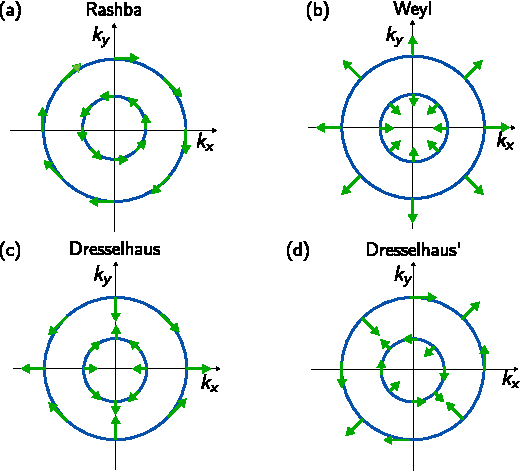
\includegraphics{ch2/img/spin_textures.pdf}
    \caption{\textbf{Spin textures in 2DEG with different types of spin-orbit coupling.}
    The picture sketches the spin texture of a 2DEG in momentum space caused by the presence of a Rashba spin-orbit coupling term (a), a Weyl term (b), a Dresselhaus (c), and a Dresselhaus' (d).
    }
    \label{fig:spin_textures}
\end{figure}

\lipsum[11-13]

\ifSubfilesClassLoaded{%
\printbibliography
}{}
\end{document}